%!TEX root = ../main.tex
%---------------------------------------------------------------------------------------------------
%---------------------------------------------------------------------------------------------------
\FloatBarrier\section{Results}\label{Results}
%---------------------------------------------------------------------------------------------------
%---------------------------------------------------------------------------------------------------
Turning to the presentation of our results, we focus on the impact of a $\$2,000$ tuition subsidy on completed schooling and use the 90\% uncertainty set to measure the degree of uncertainty.  All our results potentially depend on the size of the uncertainty set. In practice, policy-makers choose the uncertainty set's size in line with their underlying preferences - the more desirable protection against unfavorable outcomes is, the larger the uncertainty set will be.\footnote{In a different setting, \citet{Blesch.2021} conduct an ex-ante performance evaluation  of the statistical decision functions over the whole parameter space \citep{Wald.1950,Manski.2021}.}\\

\noindent All results are based on $30,000$ draws from the asymptotic normal distribution of our parameter estimates. We follow \citet{Keane.1997} and start by analyzing the prediction for a general subsidy. Then we turn to the situation where we use endowment types for policy targeting. Throughout our analysis, we postulate a linear utility function for the policy-maker.
%---------------------------------------------------------------------------------------------------
\subsection{General subsidy}
%---------------------------------------------------------------------------------------------------
\noindent  Figure \ref{General subsidy} explores the impact prediction for a general tuition subsidy. We show the point prediction, its sampling distribution, and the uncertainty set. At the point estimate, average schooling increases by $0.65$ years. However, there is considerable uncertainty about the prediction, as the uncertainty set ranges from $0.15$ to $1.10$ years.\\

\begin{figure}[ht!]\centering
\scalebox{0.35}{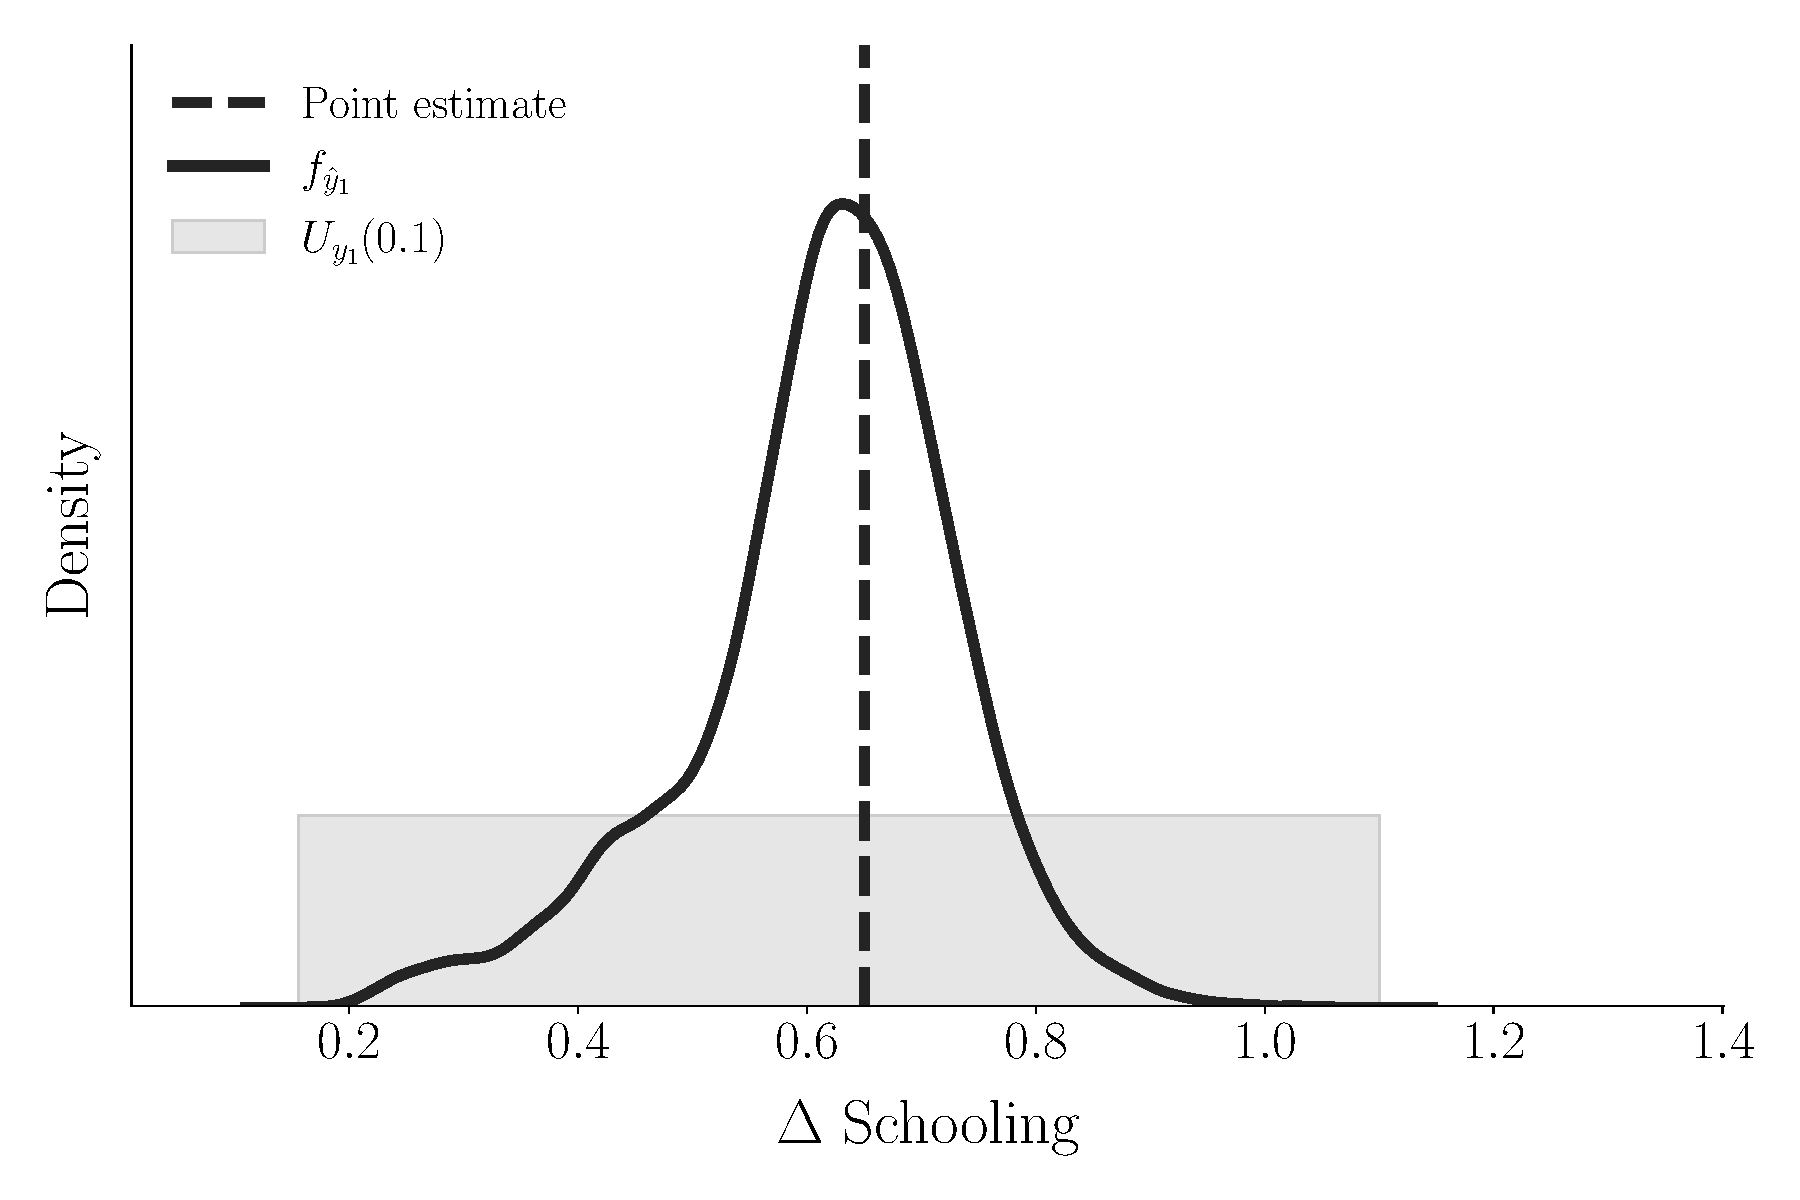
\includegraphics{fig-policy-average-years-bw}}
\caption{General subsidy}\label{General subsidy}
\end{figure}\FloatBarrier
%
\noindent In Figure \ref{Time preference}, we trace the effect of the discount rate $\delta$ on the subsidy's impact over the uncertainty set, while keeping all other parameters at their point estimate. Initially, as  $\delta$ increases, so does the policy's impact as individuals value the long-term benefits from increasing their level of schooling more and more. However, for high levels of the discount factor, the policy's impact starts to decrease as most individuals already complete a high school or college degree even without the subsidy.
%
\begin{figure}[ht!]\centering
\scalebox{0.35}{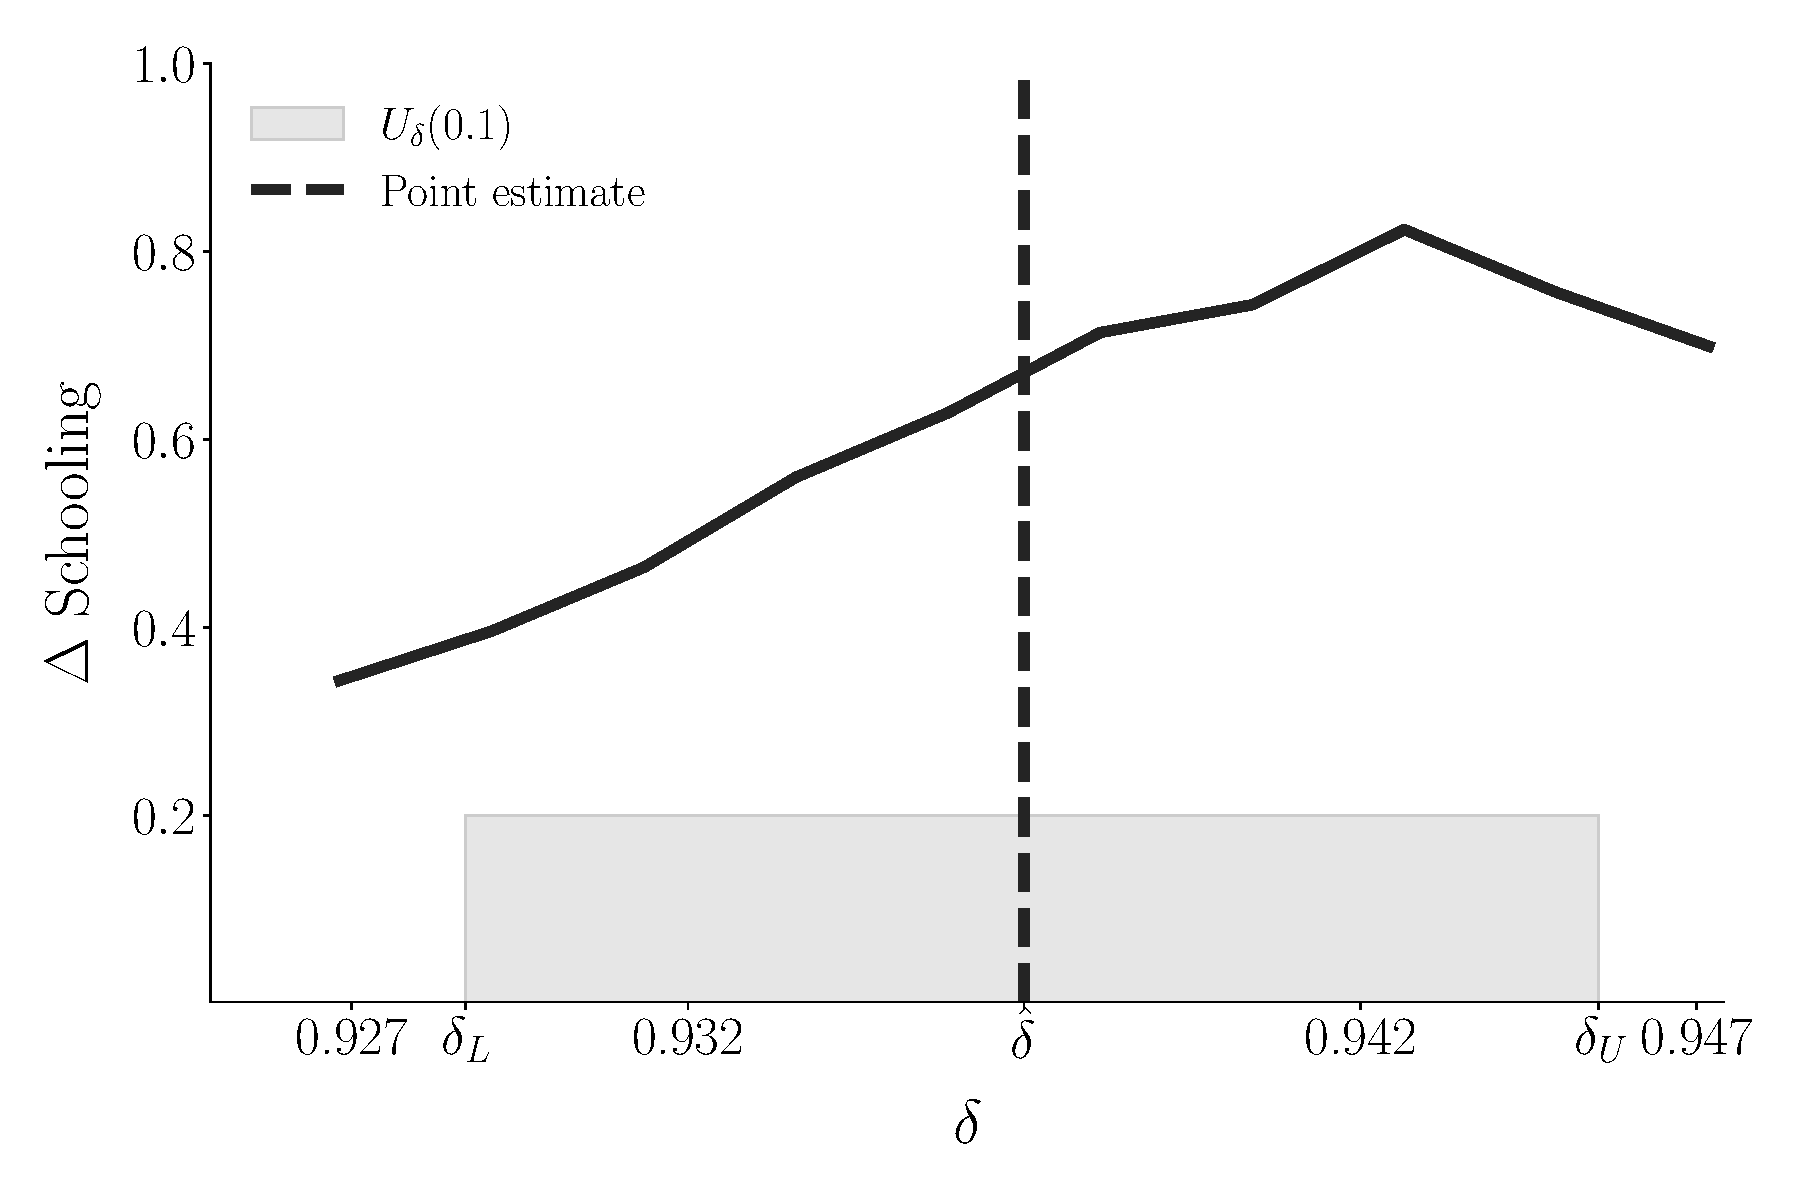
\includegraphics{fig-trace-delta-bw}}
\caption{Time preference}\label{Time preference}
\end{figure}\FloatBarrier
%---------------------------------------------------------------------------------------------------
\subsection{Targeted subsidy}
%---------------------------------------------------------------------------------------------------
So far, we restricted the analysis to a general subsidy available to the whole population and the average predicted impact. We now examine the setting in which a policy-maker can target individuals based on the type of their initial endowment. The importance of early endowment heterogeneity in shaping economic outcomes over the life-cycle is the most important finding from \citet{Keane.1997}. It served as motivation for a host of subsequent research on the determinants of skill heterogeneity among adolescents \citep{Caucutt.2020,Erosa.2010,Todd.2007}.\\

\noindent To ease the exposition, we initially focus our discussion of results on Type 1 and Type 3 individuals. We later rank policies targeting either of the four types based on the different decision-theoretic criteria. Additional results are available in our Appendix.\\

\noindent Figure \ref{Type heterogeneity} confirms that life-cycle choices differ considerably by initial endowment type. On the left, we show the number of periods the two types spend on average in each of the five alternatives. Those characterized as Type 1 individuals spend more than six years on their education even after entering the model. Type 3 individuals, on the other hand, extend their academic pursuits for only an additional two years. This difference translates into very different labor market experiences. While Type 1 individuals work for about 35 years in a white-collar occupation, Type 3 workers switch more frequently between white and blue-collar occupations and spend a comparable amount of time working in either occupation -- approximately 44 years split equally among white and blue-collar occupations. Both types only spend a short time at home.
%
\begin{figure}[h!]\centering
\subfloat[Life-cycle choices]{\scalebox{0.25}{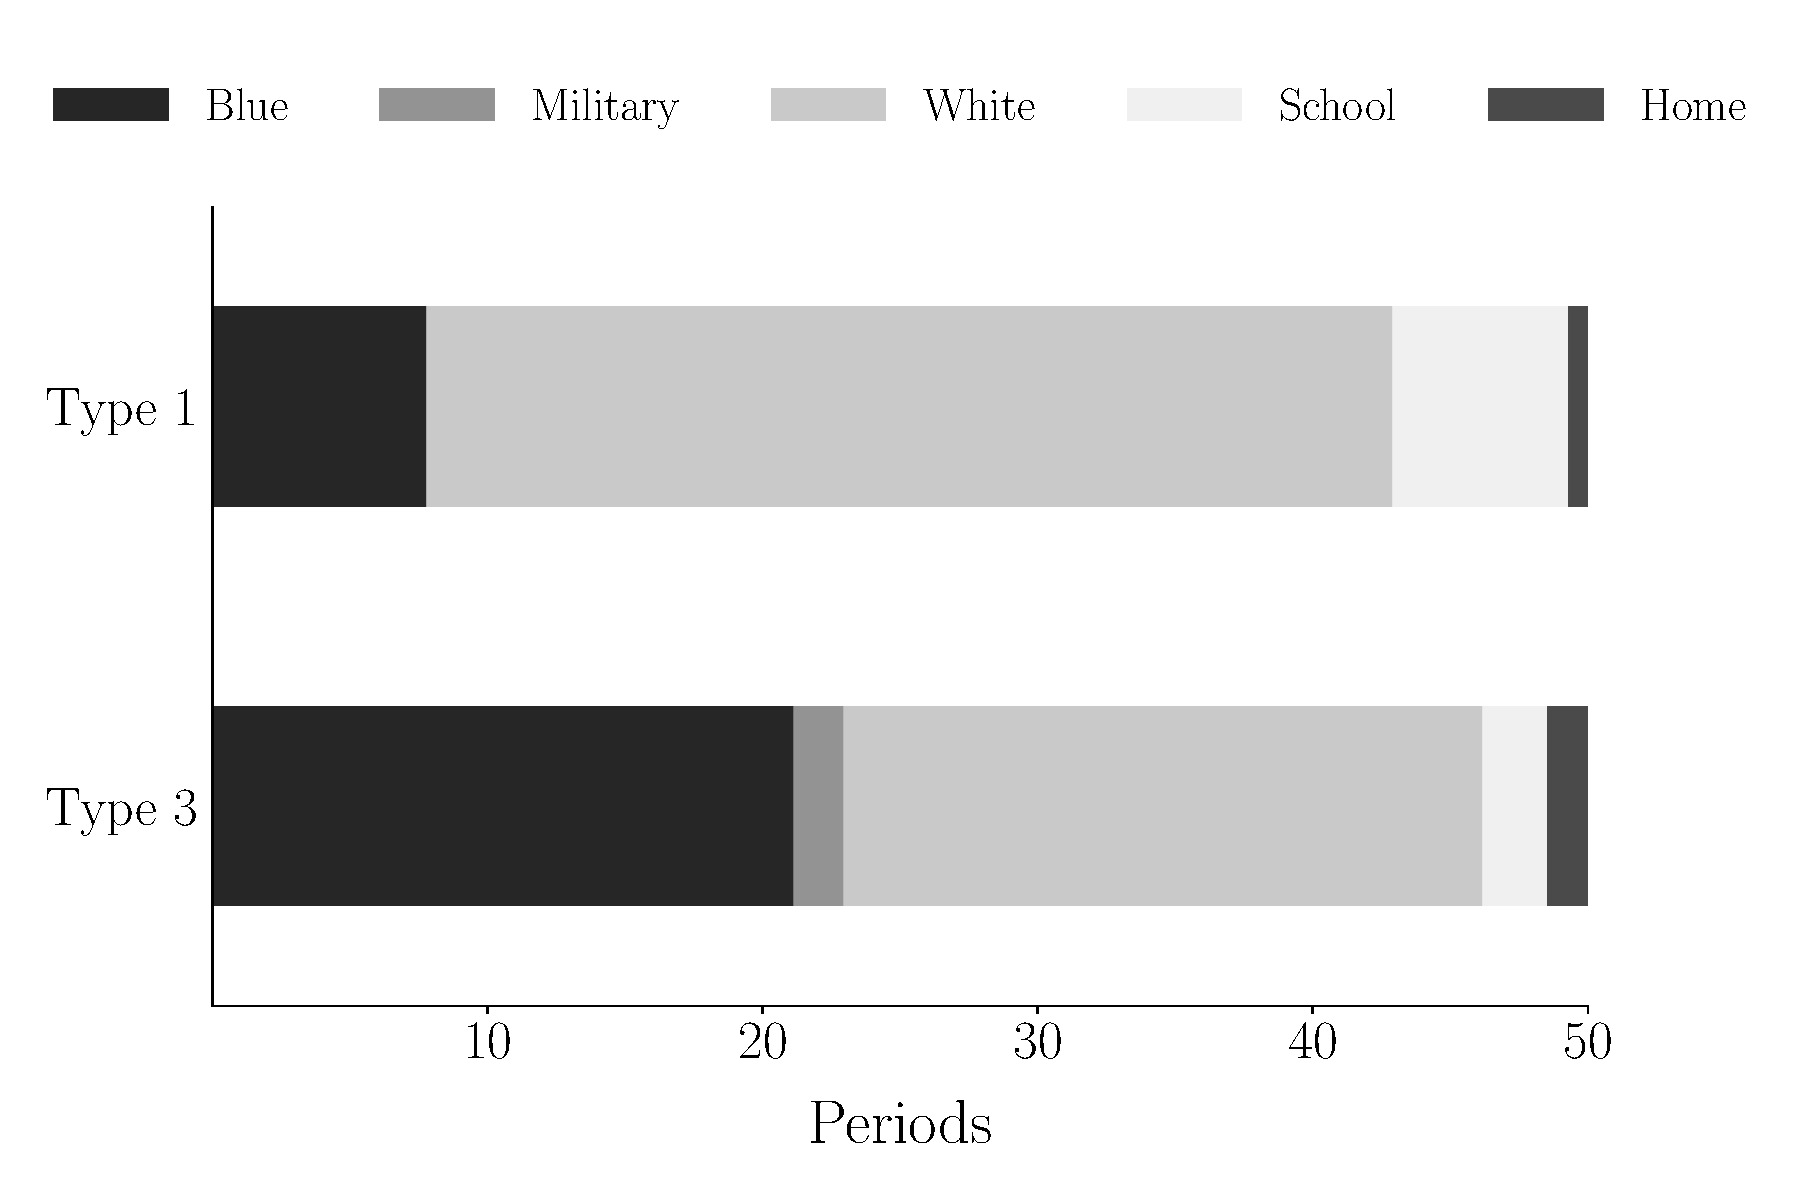
\includegraphics{fig-average-choices-by-type-bw}}\label{Type choices}}
\subfloat[Completed schooling]{\scalebox{0.25}{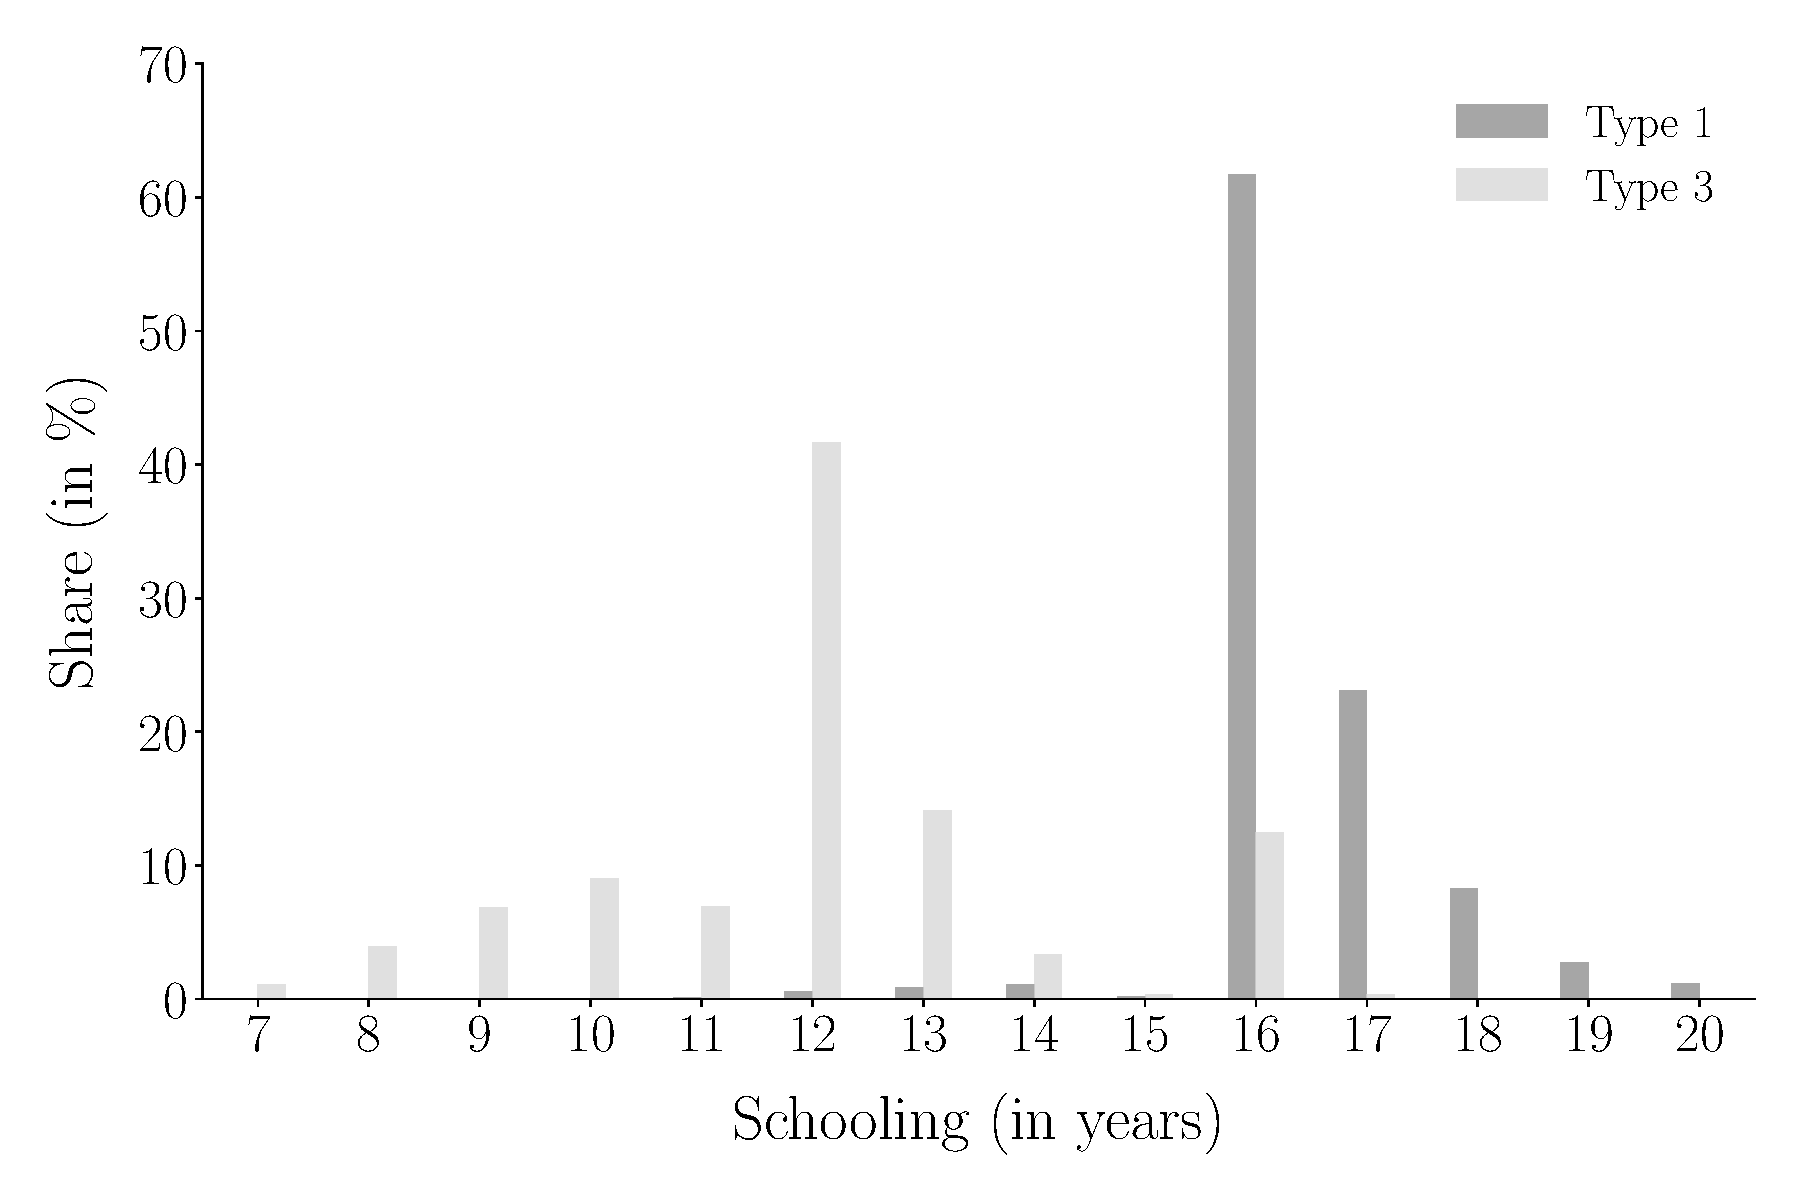
\includegraphics{fig-final-schooling-type-1-3-bw}}\label{Type schooling}}\\
\caption{Type heterogeneity}\label{Type heterogeneity}
\end{figure}\FloatBarrier
%
\noindent On the right, we show the distribution of final schooling for both types. Years of schooling are considerably higher for Type 1 individuals with an average of more than 16 years compared to only 12 years for those identified as Type 3 individuals. Nearly all Type 1 individuals enroll in college and most graduate with a degree.\\

\noindent Figure \ref{Targeted subsidy} provides a visualization of our core results for a targeted subsidy. At the point estimates, the predicted impact is considerably lower for Type 1 than Type 3. However, the prediction uncertainty is much larger for Type 3 compared to Type 1. The uncertainty set for Type 3 ranges all the way from $0$ to $1.2$ years, while the prediction for Type 1 is between $0.18$ and $0.75$.\\
%
\begin{figure}[h!]\centering
\subfloat[Type 1]{\scalebox{0.25}{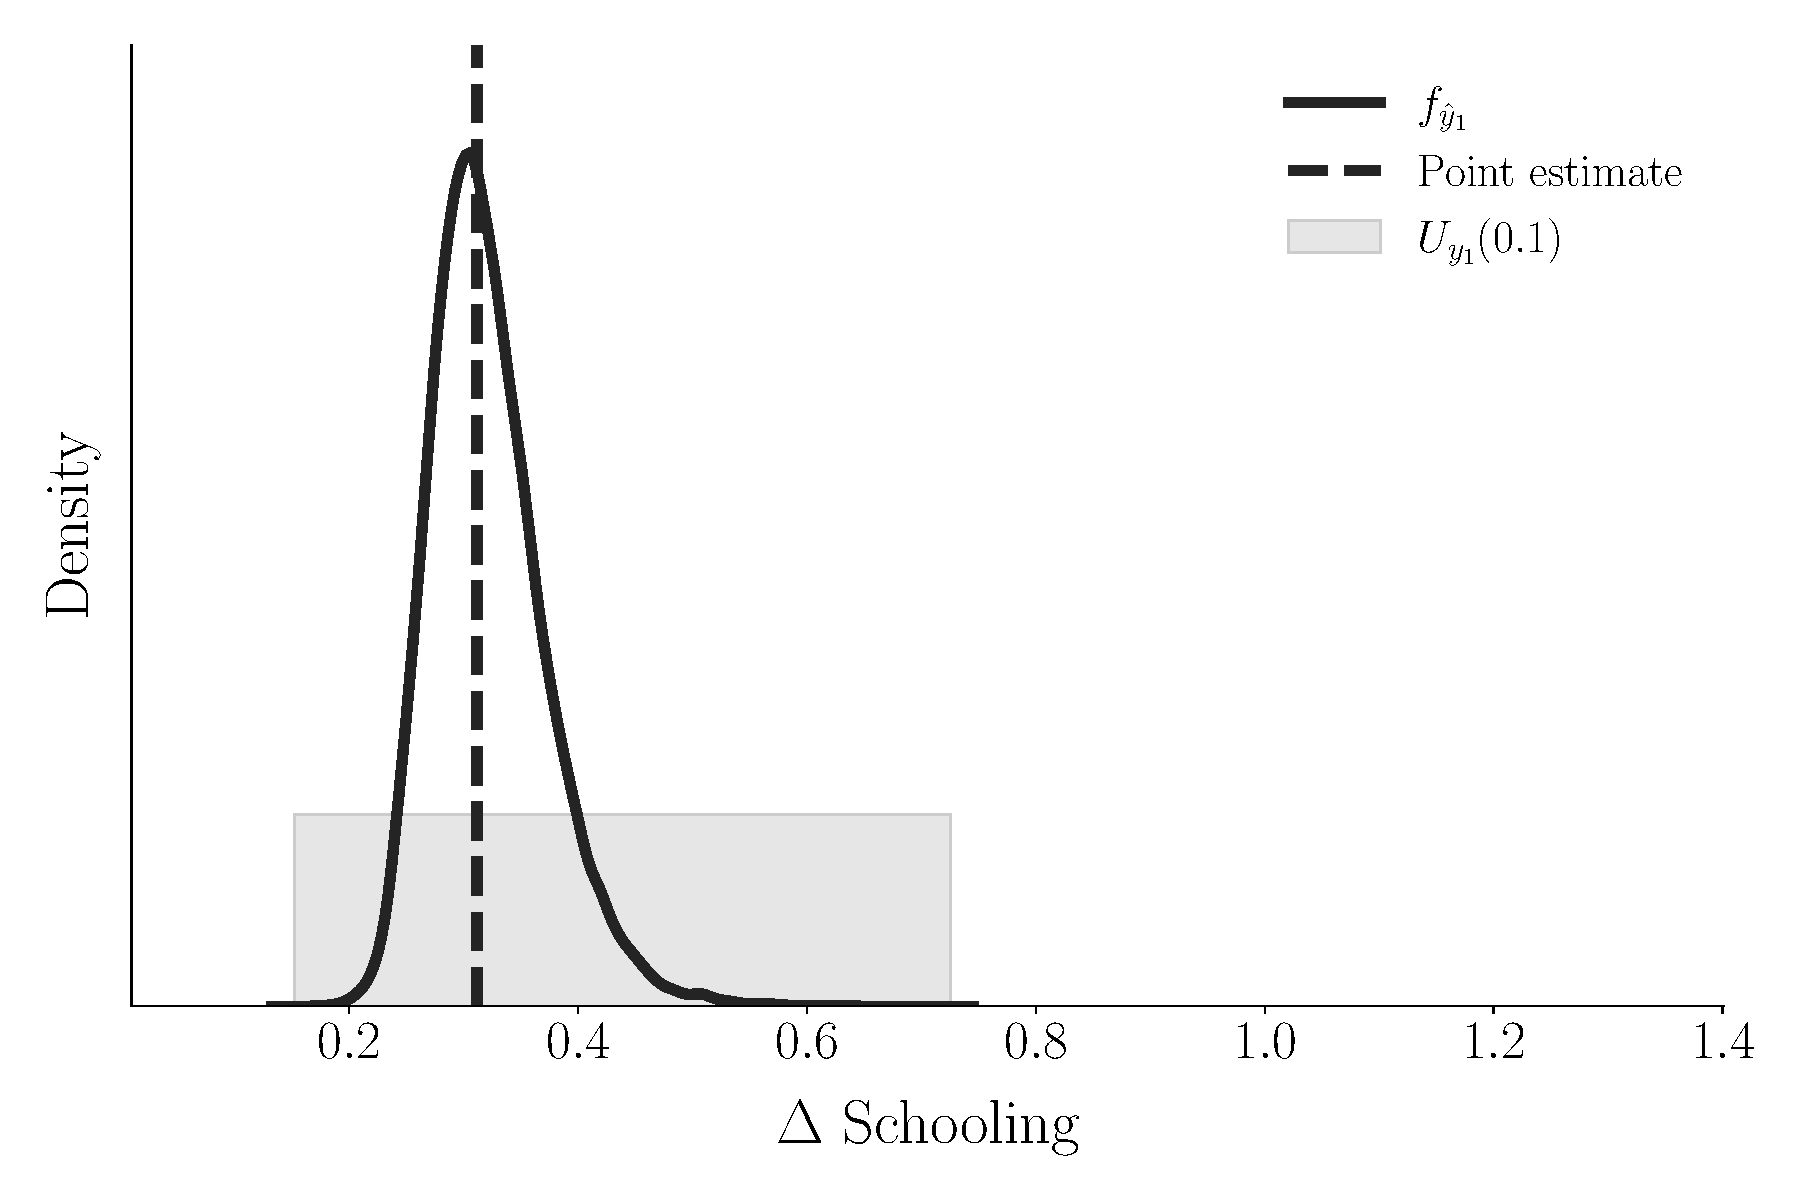
\includegraphics{fig-policy-average-years-type-0-bw}}\label{type 0}}
\subfloat[Type 3]{\scalebox{0.25}{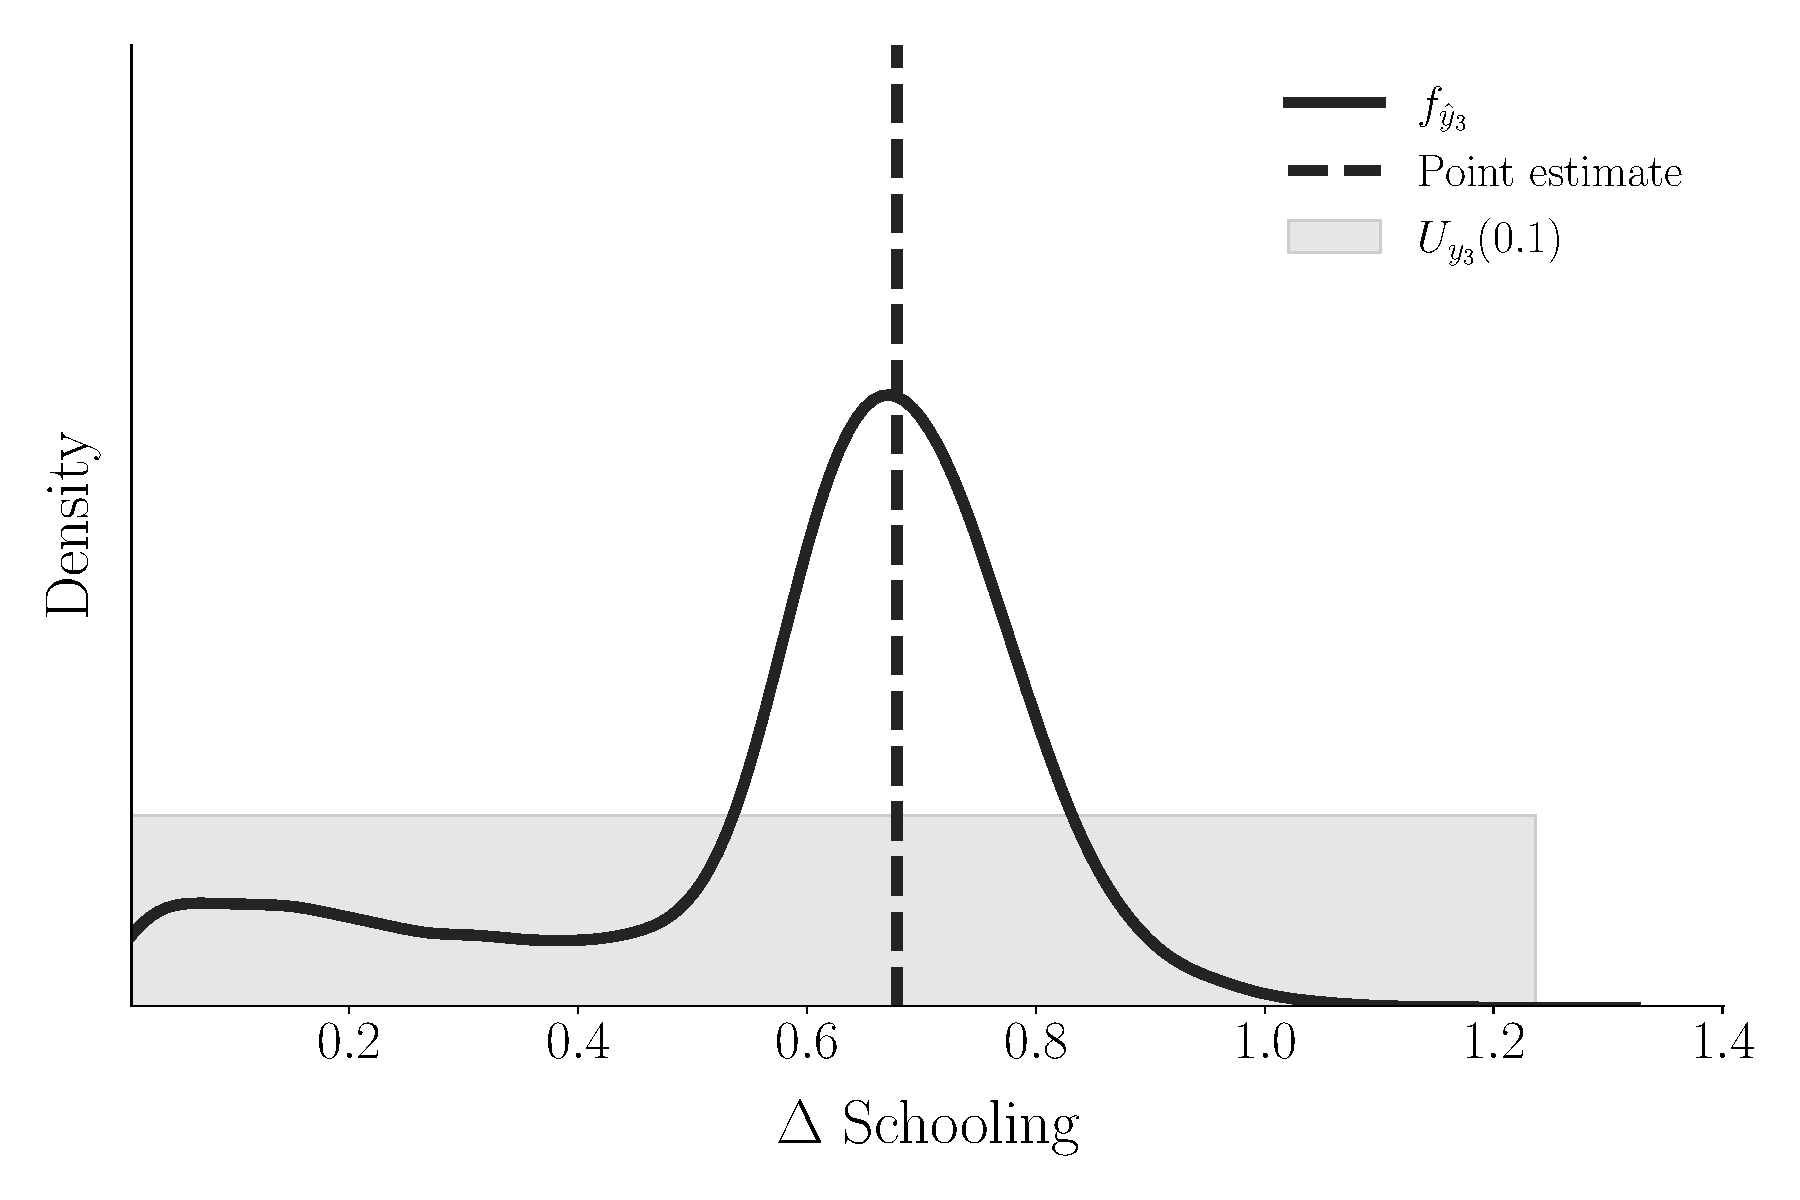
\includegraphics{fig-policy-average-years-type-2-bw}}\label{type 2}}\\
\caption{Targeted subsidy}\label{Targeted subsidy}
\end{figure}\FloatBarrier
%
\noindent This heterogeneity in impact and prediction uncertainty follows directly from the underlying economics of the model. Type 1 individuals are already more likely to have a college degree before the subsidy, and thus, the predicted impact is smaller. Alternatively, Type 1 individuals affected by the subsidy are in the middle of pursuing a college education and thus directly benefit from it. Since Type 3 individuals are at the lower end of the schooling distribution, a tuition subsidy can considerably increase their level of schooling. Whether the subsidy succeeds in doing so, however, remains uncertain.\\

\noindent We now consider the policy option to target Type 2 and Type 4 as well. Their point predictions are actually highest with an additional $0.81$ years on average for Type 2 and $0.75$ years for Type 4. However, both predictions are fraught with uncertainty. For Type 2 the uncertainty set ranges from $0.17$ to $1.3$, while for Type 4 it starts at zero and spans all the way to $1.18$.\\

\noindent Figure \ref{Ranking} shows the policy alternative's ranking by the decision-theoretic criteria we discussed in Section \ref{Statistical decision theory}. Ranking alternatives using as-if optimization is straightforward. A policy targeting Type 2 is the most preferred alternative, while a focus on Type 1 is the least attractive. However, once we account for the presence of uncertainty in the predictions, a more nuanced picture emerges. Moving from as-if optimization to a subjective Bayes criterion using a uniform distribution over the uncertainty set does not change the ordering. However, once a decision-maker is concerned with performance across the whole range of values in the uncertainty set -- we move to the minimax regret or maximin criterion -- a policy targeting Type 1 becomes more and more attractive despite its low point prediction because its worst-case utility is highest.\\
%
\begin{figure}[h!]\centering
\scalebox{0.35}{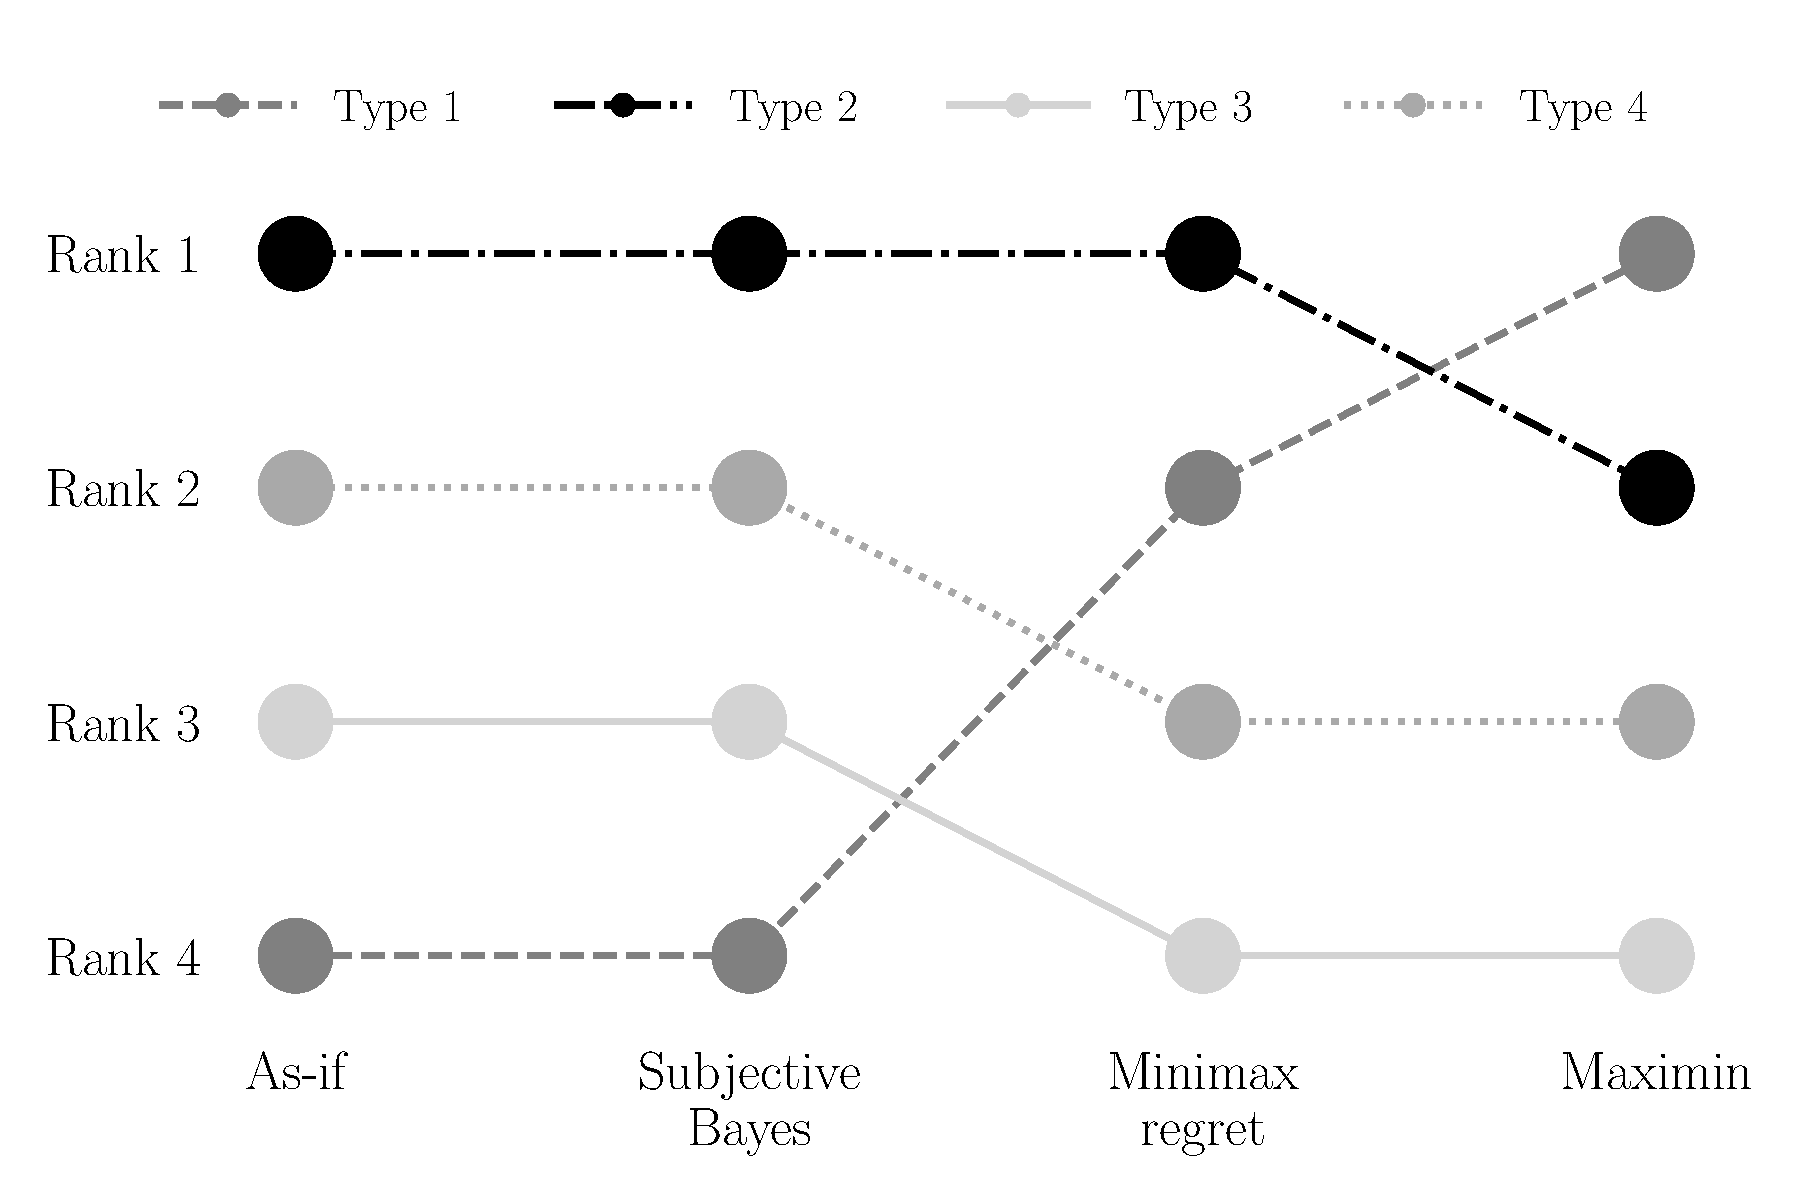
\includegraphics{fig-criterion-policy-ranks-bw}}
\caption{Policy ranking}\label{Ranking}
\end{figure}\FloatBarrier
%
\noindent In general, framing policy advice as a decision problem under uncertainty shows that there are many different ways of making reasonable decisions. The ranking of policies varies depending on the decision criteria. Not only that, but due to the necessary ex-post nature of our implementation, the ranking for a given criteria also depends on the choice of $\alpha$. The selection of $\alpha$ is part of the decision problem: the more a policy-maker is concerned about worst-case scenarios, the smaller the appropriate value for $\alpha$ will be. After deciding on a preferred decision rule, we suggest performing a sensitivity analysis around the selected $\alpha$ value by checking how much the policy ranking varies within a neighborhood.
